\chapter{Prozesserstellung}
Der Architekturprozess ist komplex und ein falsches Vorgehen kann der Ursprung vieler Probleme sein \cite[S. 7-8]{softarch}. Deswegen ist es notwendig einen eigenen Prozess zu definieren, welcher die Erstellung vereinfacht und die Fehlerkosten minimiert. Dieser Prozess soll schon in der Planungsphase zum Einsatz kommen, da hier wegen der 10er Regel der Fehlerkosten der Größte Effekt zur Reduzierung der Fehlerkosten erzielt werden kann \cite[S. 154]{fehler}.

Dieser Prozess wurde anhand eines Beispielprojektes erstellt und dreht sich um die Architektur eines Systems einer Zertifizierungsstelle.

In diesem Kapitel wird der Weg zur Erstellung des Prozesses beschrieben und erklärt, warum die die initial vermuteten nicht funktionalen Anforderungen nicht geeignet für die initiale Aufspaltung des Systems sind.

\section{Vorhandene Daten}
Ausgegangen wurde von folgenden Anforderungsdokumenten, welche in der Erstellung des Prozesses mehrfach abgeändert und an die Architekturprozessanforderungen angepasst wurden:

\begin{itemize}
  \item Usecasediagramm: modelliert die Usecases des Unternehmens
  \item Usecasebeschreibung: ausgefülltes Anforderungstemplate, welches Sonderfälle, nicht funktionale Parameter und weitere Details beinhaltet
  \item Klassendiagramm: visualisiert die zu verwendeten Daten
  \item Aktivitätsdiagramme: visualisiert den Ablauf komplexerer Usecases
  \item Kontextdiagramm: zeigt die Datenflüsse zwischen AkteurInnen, Nachbarsystemen und dem zu erstellenden System
  \item ISO Anforderungsdokument für Zertifizierungsstellen \cite{ISO_CERT}: beschreibt die Rahmenbedingungen für den Betrieb einer Zertifizierungsstelle
\end{itemize}


\section{Prozesserstellungsversuche}
Ausgehend von den vorhandenen Daten wurden mehrere Prozesse definiert, welche bis auf den Letzten entweder zu grobe Ergebnisse lieferten, oder nicht nachvollziehbar waren.

Ausgangsbasis war eine Systemvision mit folgenden Anforderungen:

\begin{itemize}
  \item Es soll eine Webseite entstehen, welche die Prüfungstermine auflistet und Personen erlaubt, sich für diese Prüfungen anzumelden
  \item Die Übermittlung der Prüfungsdaten soll über einen eigenen VPN Server geschehen
  \item Die Prüfungsdaten werden firmenintern verwaltet und nach der Auswertung soll der Scheme Owner benachrichtigt werden
\end{itemize}

\begin{figure}[!htbp]
    \centering
    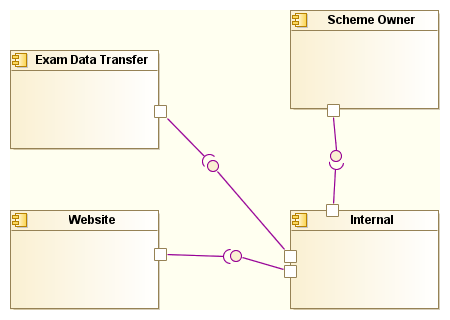
\includegraphics[scale=0.6]{uml/vision.png}
    \caption{Systemvision der Komponenten}
\end{figure}

Aufbauend darauf wurde dann versucht einen Prozess zu finden, der diese Grundideen berücksichtigt.

\subsection{Vom Usecase zur Komponente}
Der erste Versuch zur Erstellung des Architekturprozesses orientierte sich am Prinzip: teile und herrsche. Der Prozess hing aufgrund der initialen starken Gewichtung der nicht funktionalen Anforderungen stark von diesen ab und sollte auf folgender Weise funktionieren:

\begin{itemize}
  \item Für jeden Usecase wird ein komplettes Komponentendiagramm des Systems erstellt
  \item Die Komponenten jedes Teilsystems werden anhand ihrer nicht funktionalen Qualitäten aus einem Pool von Komponentenarchitekturen gewählt. Diese Komponentenarchitekturen beinhalteten zB. Systeme wie den üblichen Webstack, welcher sich aus Komponenten wie dem Loadbalancer, Datenbankserver, Applikationsserver und Webserver zusammensetzt.
  \item Schlussendlich werden alle Teilsysteme mit einander vereinigt, soweit es die nicht funktionalen Attribute erlauben
\end{itemize}

Dieser Prozess scheiterte nicht nur am enormen Modellierungsaufwand, sondern auch am Auswahlprozess der Komponentenarchitekturen: Je nachdem, welche Komponentenarchitekturen vorhanden waren und wie diese bewertet wurden, entstanden unterschiedliche Architekturen. Zudem schien es zu viele Komponentenarchitekturen zu geben, da die einzelnen Komponenten beliebig miteinander kombinierbar waren.

Die Qualität der Architektur hätte folglich von der Vollständigkeit dieser scheinbar unendlich großen Menge an Komponentenarchitekturen abgehangen. Aus diesem Grund schien er ungeeignet und wurde verworfen.

\subsection{Von einer erweiterten Systemvision auf eine verfeinerte Architektur durch nicht funktionale Anforderungen}
Um das Problem des sehr hohen Modellierungsaufwandes des ersten Prozesses zu umgehen, wurde von einer erweiterten Systemvision in Form eines Komponentendiagrammes ausgegangen. Diese Komponentenarchitektur entstand zusammen mit dem/der AuftraggeberIn.

\begin{figure}[!htbp]
    \centering
    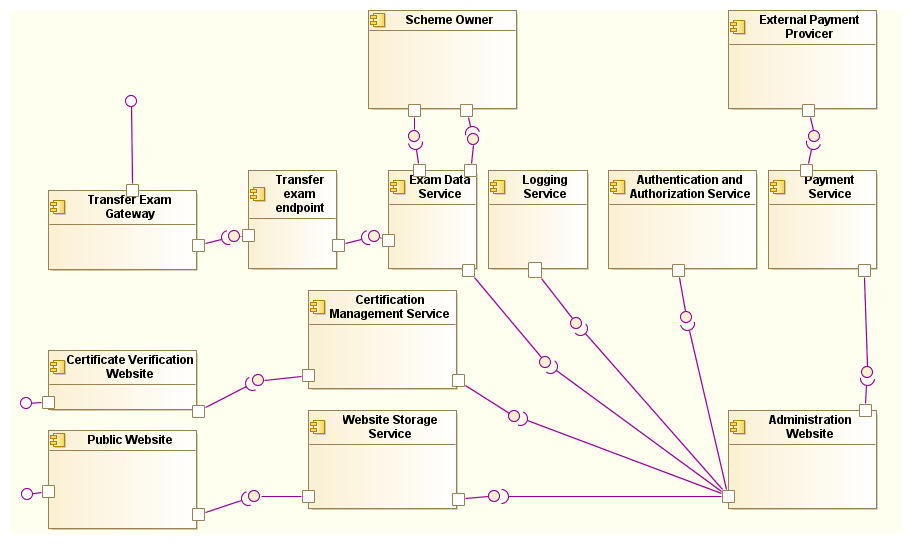
\includegraphics[scale=0.5]{uml/vision2.png}
    \caption{Erweiterte, geschätzte Systemvision der Komponenten}
\end{figure}

Diese Architektur sollte nun anhand der nicht funktionalen Anforderungen jedes Usecases angepasst werden.

Auch dieser Prozess litt jedoch unter dem Problem, dass die nicht funktionalen Anforderungen schwer bewertet werden konnten. Über dies hinaus war es schwer ein Regelwerk/Rezept aus der Architekturerstellung abzuleiten, da durch die Einbeziehung unterschiedlicher AuftraggeberInnen jeweils verschiedene Architekturen entstehen können.

\subsection{Von den Daten zur Architektur}
Die Auswahl und Bewertung der Komponentenarchitekturen und der starke Fokus auf die nicht funktionalen Anforderungen in den vorherigen beiden Prozessen stellte ein wesentliches Hindernis zur Erstellung eines eindeutigen Regelwerkes dar. Eine vollständige Auflistung aller möglichen Komponentenarchitekturen erschien entweder als unmöglich oder unvollständig; eine Bewertung der nicht funktionalen Attribute schien ohne entsprechende Implementation nur sehr grob überprüfbar zu sein.

Da sich dieser Prozess jedoch ausschließlich auf die Planungs- und nicht die Implementationsphase bezieht, wurden die nicht funktionalen Anforderungen und Komponentenarchitekturen als Hauptkriterium und Ausgangspunkt für die Architekturerstellung verworfen.

Stattdessen wurde der Fokus auf die Aufspaltung der Daten gelegt, welche bereits schon in den Systemvisionen der vorherigen Prozesse erkennbar war.

Die Daten wurden anhand Ihrer Vertraulichkeit in unterschiedliche Zonen aufgeteilt. Diese Zonen wurden dann durch Systeme mit einander verbunden, die den Zugriff auf die Daten regelten.

\begin{figure}[!htbp]
    \centering
    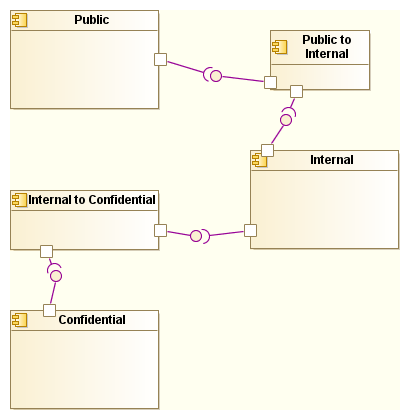
\includegraphics[scale=0.7]{uml/vision3.png}
    \caption{Aufteilung der Komponenten in Datenbereiche}
\end{figure}

Dieser Prozess erlaubte es, eine nachvollziehbare Architektur zu erstellen, jedoch war das Ergebnis zu grob. Außerdem schien eine separate Komponente zur  Übertragung der Prüfungsdaten zu fehlen, welche in der ursprünglichen Systemvision definiert und als notwendig empfunden worden war, um die Rahmenbedingungen der Vertrautheit zu erfüllen \cite[7.3]{ISO_CERT}.

\subsection{Von den Daten und den Akteuren zur Architektur}
Aufbauend auf dem vorherigen Prozess, welcher die Architektur anhand der Daten erstellte, wurden nun auch Akteure eingebunden und deren Beziehungen zu den Daten ermittelt. Anhand dieser Beziehungen wurden Regeln erstellt, aus denen wiederum die Architektur erstellt wurde.

\begin{figure}[!htbp]
    \centering
    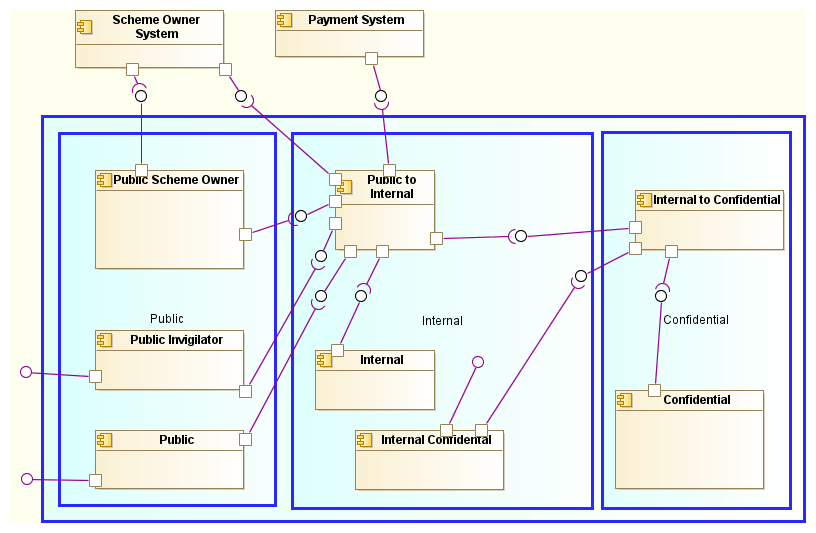
\includegraphics[scale=0.55]{uml/vision4.png}
    \caption{Aufteilung der Komponenten in Datenbereiche und Akteure}
\end{figure}

Dieser Prozess schien nicht nur die Rahmenbedingungen und Sicherheitsbedingungen abzudecken, er war auch durch die erstellten Regeln nachvollziehbar und genau genug, um bereits einen guten Überblick auf die Architektur zu erlangen. Anhand der daraus resultierenden Architektur war es nun auch möglich, nicht funktionale Attribute wie zB. Antwortzeiten besser einschätzen zu können.

Die Regeln und der Prozess im Detail befinden sich im übernächsten Kapitel. Das nächste Kapitel beschäftigt sich mit den dafür erforderlichen Anforderungensartefakten.